\documentclass[10pt]{article}

%-*-*-*-*-*-*-*-*-*-*-*-*-*-*-*-*-*-*-*Packages--*--*--*--*--*--*--*--*--*--*--*--*--*
\usepackage{amsmath}
\usepackage{tikz}
\usepackage{epigraph}
\usepackage{lipsum}
\usepackage{hyperref} 
\usepackage{listings}
\usepackage{fancyhdr}
 \usepackage[utf8]{inputenc}
\usepackage{hyperref} 
\usepackage[spanish]{babel}
%\usepackage{simpsons}
%\usepackage[dvips]{graphicx}
\usepackage{amsmath}
\usepackage{amsthm}
%\usepackage{textcomp}
\usepackage{amssymb}
\usepackage{latexsym}
\usepackage{graphicx}
%\usepackage[ansinew]{inputenc}
\usepackage{color}
%\usepackage{pstricks, pst-node, pst-plot, pst-circ}
%\usepackage{moredefs}
%\usepackage{pstricks}
%\usepackage{pst-circ}
%\usepackege{pst-node}
%\usepackage{pst-plot}
\usepackage{moredefs}
%\usepackage{mcode}
%\usepackage[above]{placeins}
\usepackage{fancybox}
\usepackage{subfig}
\usepackage{float}
%\usepackage{mcode} para colorear codigo de matlab
\usepackage{xcolor}
\usepackage{wallpaper}
\usepackage{textcomp}
%-*-*-*-*-*-*-*-*-*-*-*-*-*-*-*-*-*-*--*--*--*--*--*--*--*--*--*--*--*--*--*--*

%*****************************definiciones*******************************
\oddsidemargin -0.2in \textwidth 7.0in \topmargin -0.9in \textheight
9.0in
\parindent 3em
\hyphenation{e-jem-plo
e-rro-res de-pen-dien-te co-rrien-te res-pues-ta fi-gu-ran
cons-tan-tes o-pe-ra-cion i-lu-mi-na-cion}

\pagestyle{fancy}
\headheight 50pt 
\renewcommand{\arrayrulewidth}{3pt} 
\newtheorem{defi}{{\it Definición}}[section]
%@@@@@@@@@@@@@@@@@@@@@@@@@@@cabecera y pie de pagina @@@@@@@@@@@@@@@@@@@@@@@@@@@@@@@@@@@@@@@@@@@@@@@@@@@@@@

\rhead{
\includegraphics[width=.075\textwidth]{./Images/logo_iaci2.eps}}
\chead{}
\lhead{Teoría de las Telecomunicaciones}
\rfoot{1º cuatrimestre 2015  }
\cfoot{\thepage}
\lfoot{\bf{Universidad Nacional de Quilmes}}
%@@@@@@@@@@@@@@@@@@@@@@@@@@@@@@@@@@@@@@@@@@@@@@@@@@@@@@@@@@@@@@@@@@@@@@@@@@@@@@@@@@@@@@@@@@@@@@@@@@@@@@@@@@@

%::::::::::::::::::::::Colores varios:::::::::::::::::::::::::::::::::::::::::::::::::::::::::::::::::::::::

\definecolor{azul-claro}{rgb}{0.335,0.89,1}
\definecolor{gainsboro}{rgb}{0.86,0.86,0.86}
\definecolor{mediumseagreen}{rgb}{0.24,0.7,0.44}
\definecolor{moccasin}{rgb}{1,0.89,0.71}
\definecolor{cornflowerblue}{rgb}{0.39,0.58,0.93}
\definecolor{lightgray}{rgb}{0.83,0.83,0.83}
\definecolor{darkgrey}{rgb}{0.66,0.66,0.66}
\definecolor{darkslategray}{rgb}{0.18,0.31,0.31}
\definecolor{lavender}{rgb}{0.9,0.9,0.98}
\definecolor{azure}{rgb}{0.94,1,1}
\definecolor{honeydew}{rgb}{0.94,1,0.94}

%:::::::::::::::::::::::::::::::::::::::::::::::::::::::::::::::::::::::::::::::::::::::::::::::::::::::::::::
%Requiere \usepackage{xcolor}
\renewcommand{\arrayrulewidth}{1pt} 
\newcommand{\mcaja}[1]{%
{{\fboxsep 10pt \fboxrule 1pt%
\fcolorbox{black}{orange}{%
\color{black} \Huge #1}}}
}
\newcommand{\nuevobox}[1]{%
{{\fboxsep 14pt \fboxrule 1pt%
\fcolorbox{black}{darkgrey}{%
\color{lavender} \huge #1}}}
}
\newcommand{\ssection}[1]{\section[#1]{\mcaja{#1}}}
\makeatletter
\newcommand{\sect}[1]{\subsection[#1]{\nuevobox{#1}}}
\makeatletter
\def\section{\@ifstar\unnumberedsection\numberedsection}
\def\numberedsection{\@ifnextchar[%]
\numberedsectionwithtwoarguments\numberedsectionwithoneargument}
\def\unnumberedsection{\@ifnextchar[%]
\unnumberedsectionwithtwoarguments\unnumberedsectionwithoneargument}
\def\numberedsectionwithoneargument#1{\numberedsectionwithtwoarguments[#1]{#1}}
\def\unnumberedsectionwithoneargument#1{\unnumberedsectionwithtwoarguments[#1]{#1}}
\def\numberedsectionwithtwoarguments[#1]#2{%
\ifhmode\par\fi
\removelastskip
\vskip 3ex\goodbreak
\refstepcounter{section}%
\begingroup
%\noindent
\leavevmode\large\bfseries\raggedright\mcaja%%
\thesection\ #2\par\nobreak
\endgroup
\noindent\hrulefill\nobreak
\vskip 2ex\nobreak
\addcontentsline{toc}{section}{%
\protect\numberline{\thesection}%
#1}%
}
\def\unnumberedsectionwithtwoarguments[#1]#2{%
\ifhmode\par\fi
\removelastskip
\vskip 3ex\goodbreak
% \refstepcounter{section}%
\begingroup
\noindent
\leavevmode\Large\bfseries\raggedright
% \thesection\
#2\par\nobreak
\endgroup
\noindent\hrulefill\nobreak
\vskip 0ex\nobreak
\addcontentsline{toc}{section}{%
%
\protect\numberline{\thesection}%
#1}%
}
\makeatother
%%%Cap\’itulos
\usepackage{helvet}
%\usepackage{psboxit,pstcol}
\makeatletter
\def\@makechapterhead#1{%
{\parindent \z@ \raggedright \reset@font
\hbox to \hsize{%
\rlap{\raisebox{-2.5em}{\raisebox{\depth}{%%% Necesita la imagen "imgCapitulo"

\includegraphics[width=10em]{./Images/logo_iaci2.eps}}}}%
\rlap{\hbox to 6em{\hss
\reset@font\sffamily\fontsize{8em}{8em}\selectfont\black
\thechapter\hss}}%
\hspace{10em}%
\vbox{%
\advance\hsize by -10em
\reset@font\fontfamily{hv}\bfseries\Large
#1
\par
}%
}}%
\vskip 5pt
\hrulefill
\vskip 50pt
}
\makeatother
%----------------------------------------------------------------------------------------
% Theorems
\newtheorem{theorem}{Teorema}[section]
\newtheorem{corollary}{Corolario}[theorem]
\newtheorem{lemma}[theorem]{Lema}
%----------------------------------------------------------------------------------------


%----------------------------------------------------------------------------------------
%	TITLE PAGE
%----------------------------------------------------------------------------------------
\definecolor{titlepagecolor}{cmyk}{1,.73,0,.37}


\newcommand\titlepagedecoration{%
\begin{tikzpicture}[remember picture,overlay,shorten >= -10pt]

\coordinate (aux1) at ([yshift=-15pt]current page.north east);
\coordinate (aux2) at ([yshift=-410pt]current page.north east);
\coordinate (aux3) at ([xshift=-4.5cm]current page.north east);
\coordinate (aux4) at ([yshift=-150pt]current page.north east);

\begin{scope}[titlepagecolor!40,line width=12pt,rounded corners=12pt]
\draw
  (aux1) -- coordinate (a)
  ++(225:5) --
  ++(-45:5.1) coordinate (b);
\draw[shorten <= -10pt]
  (aux3) --
  (a) --
  (aux1);
\draw[opacity=0.6,titlepagecolor,shorten <= -10pt]
  (b) --
  ++(225:2.2) --
  ++(-45:2.2);
\end{scope}
\draw[titlepagecolor,line width=8pt,rounded corners=8pt,shorten <= -10pt]
  (aux4) --
  ++(225:0.8) --
  ++(-45:0.8);
\begin{scope}[titlepagecolor!70,line width=6pt,rounded corners=8pt]
\draw[shorten <= -10pt]
  (aux2) --
  ++(225:3) coordinate[pos=0.45] (c) --
  ++(-45:3.1);
\draw
  (aux2) --
  (c) --
  ++(135:2.5) --
  ++(45:2.5) --
  ++(-45:2.5) coordinate[pos=0.3] (d);   
\draw 
  (d) -- +(45:1);
\end{scope}
\end{tikzpicture}%
}


\newcommand*{\plogo}{\fbox{$\mathcal{PL}$}}
\newcommand*{\titleGP}{\begingroup % Create the command for including the title page in the document
\centering % Center all text
\vspace*{\baselineskip} % White space at the top of the page

\rule{\textwidth}{1.6pt}\vspace*{-\baselineskip}\vspace*{2pt} % Thick horizontal line
\rule{\textwidth}{0.4pt}\\[\baselineskip] % Thin horizontal line

{\LARGE Teoría de las telecomunicaciones\\[0.3\baselineskip] Laboratorio 1}\\[0.2\baselineskip] % Title

\rule{\textwidth}{0.4pt}\vspace*{-\baselineskip}\vspace{3.2pt} % Thin horizontal line
\rule{\textwidth}{1.6pt}\\[\baselineskip] % Thick horizontal line

\scshape % Small caps
 Martín Noblía 
\vspace*{2\baselineskip} % Whitespace between location/year and editors

Profesores: \\[\baselineskip]
{\Large Fabian Iakinchuk\\ Martín Castillo\par}
\vfill % Whitespace between editor names and publisher logo_iaci2

\includegraphics[width=.175\textwidth]{./Images/logo_iaci2.eps}

% Editor list
{\itshape Universidad Nacional de Quilmes \par} % Editor affiliation

\vfill % Whitespace between editor names and publisher logo

%\plogo \\[0.3\baselineskip] % Publisher logo
{\scshape 2015} \\[0.3\baselineskip] % Year published
%{\large THE PUBLISHER}\par % Publisher

\endgroup}

%----------------------------------------------------------------------------------------
%	BLANK DOCUMENT
%----------------------------------------------------------------------------------------


\begin{document}
\pagestyle{empty} 

\titleGP

\titlepagedecoration

\newpage
\pagestyle{fancy}

\section{Problema 1}

Dada una fuente de datos en un archivo de texto nombrado:\verb|texto.txt|.
Escribir un algoritmo de manera tal que calcule la probabilidad de ocurrencia 
de cada símbolo existente en la fuente.
Mostrar en un listado (sea en pantalla o en otro archivo \verb|.txt| cada 
elemento de la fuente con su probabilidad calculada asociada.
Calcular la entropía de la fuente.
\subsection{resolución}
Para resolver este problema utilizamos el lenguaje de programación Julia(\url{http://www.julialang.org})
el cual es \textit{opensource}, dinámico y tiene velocidades de procesamiento relativas a C entre otras 
caracteristicas.

El script que realiza la tarea es el siguiente:

\begin{verbatim}
#= Script para el problema 1
desde consola:
julia problema1.jl
=#
# incluimos el modulo
include("teleco.jl")
# leemos el archivo
T = open(readall,"../Archivos/texto.txt");
# calculamos las frecuencias y probabilidades 
d,p = Teleco.probs(T[1:end-1]);
# Mostramos los resultados
Teleco.show_source(d)
# Calculamos la entropia de la fuente
h = Teleco.entropy(p);
print("La fuente discreta texto.txt tiene una entropia: $h [bits/simbolo]")
\end{verbatim}

Las definiciones de funciones estan agrupadas en el modulo \verb|Teleco|
que esta definido en el archivo \verb|teleco.jl|. El cual mostramos a continuación:

\begin{verbatim}
# Modulo para el laboratorio1:Teoria de las telecomunicaciones
module Teleco
    

function probs(iter)
    # Funcion para calcular las probabilidades de ocurrencia de cada simbolo
    # en una fuente de informacion discreta sin memoria.
    # Input:
    # -----
    # iter: Cualquier fuente iterable(texto,vectores...etc) 
    # Output:
    # ------
    # d: Diccionario con los elementos de la fuente y sus frecuencias
    # p: Vector de probabilidades

    d = Dict{eltype(iter), Int}()
    l = length(iter)
    
    for e in iter
        d[e] = get(d, e, 0) + 1 
    end
    p = collect((values(d))) / l 
    return d,p
end

function freqs_pr(iter)
    # Funcion para calcular 
    pr = Collections.PriorityQueue()
    
    for e in iter
        pr["$e"] = get(pr, "$e", 0) + 1 
    end
    
    return pr
end


function entropy(p)
   # Funcion para calcular la entropia de una 
   # fuente discreta sin memoria
   # Input:
   # -----
   # p: Vector de probabilidades de la fuente
   # Output:
   # ------
   # h: Entropia de la fuente
    i = log2(1./p)
    aux = p.*i
    h = sum(aux)
    
    return h

end

function show_source(d)
    # Funcion para mostrar los elementos de una fuente 
    # y su frecuencia de aparicion
    for (v,k) in zip(values(d),keys(d))
        println("elemento: $k --> frecuencia: $v")
    end
end    

export probs, probs_pr,entropy, show_source


end

\end{verbatim}

Cuya salida es:

\begin{verbatim}

elsuizo@debian:~/Telecomunicaciones/Laboratorios/Lab1/Programas/Julia$ ~/julia/./julia problema1.jl 
elemento: á --> frecuencia: 4
elemento: l --> frecuencia: 6
elemento: m --> frecuencia: 2
elemento: r --> frecuencia: 5
elemento: f --> frecuencia: 1
elemento: o --> frecuencia: 3
elemento: t --> frecuencia: 2
elemento: a --> frecuencia: 14
elemento: E --> frecuencia: 1
elemento: v --> frecuencia: 2
elemento: n --> frecuencia: 5
elemento: e --> frecuencia: 13
elemento: w --> frecuencia: 2
elemento: h --> frecuencia: 3
elemento: d --> frecuencia: 3
elemento: c --> frecuencia: 2
elemento: ; --> frecuencia: 1
elemento: p --> frecuencia: 2
elemento: i --> frecuencia: 4
elemento: q --> frecuencia: 5
elemento: s --> frecuencia: 4
elemento: u --> frecuencia: 8
La fuente discreta texto.txt tiene una entropia: 4.066909301939965 [bits/simbolo]
\end{verbatim}


\section{Problema 2}

Dado un archivo de texto nombrado “texto2.txt” el cual posee una longitud fija de
30 caracteres ASCII:

Escribir un algoritmo que codifique
cada elemento de la fuente usando codificación Huffman. (Dicha codificación puede ser
mostrada en pantalla o en un archivo de salida *.txt).
El software creado debe calcular la entropía y la longitud media del código generado.
Calcular en forma manual o con el mismo software la eficiencia de la compresión.
Verifique si el código generado es óptimo.

\subsection{resolución}


\newpage

\section{Problema 3}
Dado dos archivos de texto llamados Castellano.txt e ingles.txt, los cuales están en
diferente lenguaje, comprimir los mismos en formato ZIP y:
\begin{itemize}
\item a- Realizar una tabla donde se pueda visualizar el cociente entre: (tamaño nuevo /
tamaño original) x100.
\item b- Realizar una tabla con la probabilidad de ocurrencia de cada uno de los caracteres
para cada texto.
\item c- Analizar los resultados de a) y b). Sacar conclusiones.
\end{itemize}

\subsection{resolución}

Para la resolver este problema utilizamos un script en el lenguaje Julia, cuya 
salida de ejecución genera alguna de las respuestas. A continuación los códigos
y las salidas:

Script:

\begin{verbatim}

# Script para la resolucion del problema 3

# incluimos el modulo
include("teleco.jl")

# leemos los bytes de la fuente castellano
s1 = open(readbytes,"../Archivos/castellano.txt");
# leemos los bytes de la fuente ingles
s2 = open(readbytes,"../Archivos/ingles.txt");
# leemos los bytes de la fuente castellano zipeada
s1_zip = open(readbytes,"../Archivos/castellano.txt.zip");
# leemos los bytes de la fuente ingles zipeada
s2_zip = open(readbytes,"../Archivos/ingles.txt.zip");

# calculamos las longitudes de los archivos(bytes)
l1 = length(s1);
l2 = length(s2);
l1_zip = length(s1_zip);
l2_zip = length(s2_zip);

# calculamos los ratios
r1 = (l1_zip / l1) * 100;
r2 = (l2_zip / l2) * 100;

# mostramos los resultados
print("La eficiencia de compresión para el caso de la fuente en castellano es: $r1\n")

print("La eficiencia de compresión para el caso de la fuente en ingles es: $r2\n")

# Leemos los archivos como texto plano
Tc = open(readall,"../Archivos/castellano.txt");
Ti = open(readall,"../Archivos/ingles.txt");

# Filtramos el texto para quitar los "\n" y los espacios " "
Tc = filter!(x->(x!='\n')&&(x!=' '),collect(Tc));
Ti = filter!(x->(x!='\n')&&(x!=' '),collect(Ti));

# calculamos las frecuencias y probabilidades 
dc,pc = Teleco.probs(Tc);
d_i,p_i= Teleco.probs(Ti);
# Mostramos los resultados
println("Las frecuencias para el texto en castellano son:\n\n")
Teleco.show_source(dc)
println("Las frecuencias para el texto en ingles son:\n\n")
Teleco.show_source(d_i)
hc = Teleco.entropy(pc);
hi = Teleco.entropy(p_i);

print("La fuente discreta castellano.txt tiene una entropia: $hc [bits/simbolo]\n")
print("La fuente discreta ingles.txt tiene una entropia: $hi [bits/simbolo]\n")
\end{verbatim}

Salida del script:

\begin{verbatim}

elsuizo@debian:~/Telecomunicaciones/Laboratorios/Lab1/Programas/Julia$ ~/julia/./julia problema3.jl 
La eficiencia de compresión para el caso de la fuente en castellano es: 47.286527514231494
La eficiencia de compresión para el caso de la fuente en ingles es: 46.04361370716511
Las frecuencias para el texto en castellano son:


elemento: r --> frecuencia: 257
elemento: D --> frecuencia: 5
elemento: T --> frecuencia: 3
elemento: v --> frecuencia: 60
elemento: Y --> frecuencia: 6
elemento: y --> frecuencia: 56
elemento: d --> frecuencia: 194
elemento: c --> frecuencia: 152
elemento: I --> frecuencia: 1
elemento: g --> frecuencia: 55
elemento: p --> frecuencia: 102
elemento: i --> frecuencia: 198
elemento: q --> frecuencia: 46
elemento: S --> frecuencia: 4
elemento: : --> frecuencia: 5
elemento: á --> frecuencia: 26
elemento: f --> frecuencia: 26
elemento: ¿ --> frecuencia: 3
elemento: b --> frecuencia: 64
elemento: M --> frecuencia: 1
elemento: C --> frecuencia: 2
elemento: , --> frecuencia: 62
elemento: E --> frecuencia: 10
elemento: - --> frecuencia: 6
elemento: z --> frecuencia: 19
elemento: L --> frecuencia: 2
elemento: é --> frecuencia: 28
elemento: ú --> frecuencia: 1
elemento: s --> frecuencia: 249
elemento: t --> frecuencia: 172
elemento: a --> frecuencia: 529
elemento: P --> frecuencia: 3
elemento: x --> frecuencia: 4
elemento: ? --> frecuencia: 3
elemento: e --> frecuencia: 521
elemento: h --> frecuencia: 45
elemento: ; --> frecuencia: 6
elemento: A --> frecuencia: 6
elemento: í --> frecuencia: 19
elemento: V --> frecuencia: 1
elemento: H --> frecuencia: 1
elemento: l --> frecuencia: 225
elemento: m --> frecuencia: 125
elemento: ¡ --> frecuencia: 1
elemento: o --> frecuencia: 322
elemento: ó --> frecuencia: 30
elemento: ñ --> frecuencia: 11
elemento: U --> frecuencia: 1
elemento: ! --> frecuencia: 1
elemento: B --> frecuencia: 3
elemento: n --> frecuencia: 293
elemento: N --> frecuencia: 3
elemento: k --> frecuencia: 1
elemento: j --> frecuencia: 15
elemento: . --> frecuencia: 33
elemento: u --> frecuencia: 203
Las frecuencias para el texto en ingles son:


elemento: ' --> frecuencia: 2
elemento: r --> frecuencia: 189
elemento: D --> frecuencia: 2
elemento: T --> frecuencia: 9
elemento: v --> frecuencia: 26
elemento: Y --> frecuencia: 3
elemento: w --> frecuencia: 99
elemento: y --> frecuencia: 81
elemento: d --> frecuencia: 179
elemento: c --> frecuencia: 82
elemento: I --> frecuencia: 22
elemento: g --> frecuencia: 96
elemento: p --> frecuencia: 64
elemento: i --> frecuencia: 229
elemento: q --> frecuencia: 2
elemento: S --> frecuencia: 3
elemento: f --> frecuencia: 79
elemento: M --> frecuencia: 1
elemento: b --> frecuencia: 33
elemento: C --> frecuencia: 5
elemento: , --> frecuencia: 75
elemento: E --> frecuencia: 3
elemento: W --> frecuencia: 7
elemento: - --> frecuencia: 1
elemento: L --> frecuencia: 2
elemento: s --> frecuencia: 221
elemento: t --> frecuencia: 303
elemento: a --> frecuencia: 326
elemento: P --> frecuencia: 1
elemento: x --> frecuencia: 2
elemento: ? --> frecuencia: 3
elemento: e --> frecuencia: 424
elemento: h --> frecuencia: 224
elemento: A --> frecuencia: 13
elemento: J --> frecuencia: 1
elemento: H --> frecuencia: 7
elemento: G --> frecuencia: 2
elemento: l --> frecuencia: 178
elemento: m --> frecuencia: 102
elemento: o --> frecuencia: 320
elemento: ! --> frecuencia: 4
elemento: B --> frecuencia: 1
elemento: n --> frecuencia: 261
elemento: F --> frecuencia: 2
elemento: N --> frecuencia: 1
elemento: k --> frecuencia: 32
elemento: j --> frecuencia: 2
elemento: . --> frecuencia: 39
elemento: " --> frecuencia: 12
elemento: u --> frecuencia: 105
La fuente discreta castellano.txt tiene una entropia: 4.410238843123111 [bits/simbolo]
La fuente discreta ingles.txt tiene una entropia: 4.430201945105413 [bits/simbolo]
\end{verbatim}

\newpage


\section{Problema 4}
Se propone simular una cuantización uniforme de 4, 3 y 2 bits para una señal
sinusoidal de amplitud 1 y frecuencia 1 Hz.
\begin{itemize}
    \item a- Comparar la señal error y su relación con el número de bits de cuantizador
para 4 bits ($q=2/16$), 3 bits ($q=2/8$) y 2 bits ($q=2/8$)
    \item b- Sacar conclusiones.
\end{itemize}
\subsection{resolución}
El modulo en donde guardamos las funciones es \verb|teleco2.jl| que utilizamos posteriormente en 
el script \textit{problema4.jl}, donde comparamos la señal original $x(t) = Asin(2\pi f t)$ 
con sus versiones quantizadas uniformemente (con los distintos niveles propuestos)

A continuación su salida gráfica:


\begin{figure}[H]
   \centering
   \includegraphics[width=0.78\textwidth]{./Images/seniales_4_bits.eps}
   \caption{Cuantización 4 bits}\label{fig:q:4}     
\end{figure}


\begin{figure}[H]
   \centering
   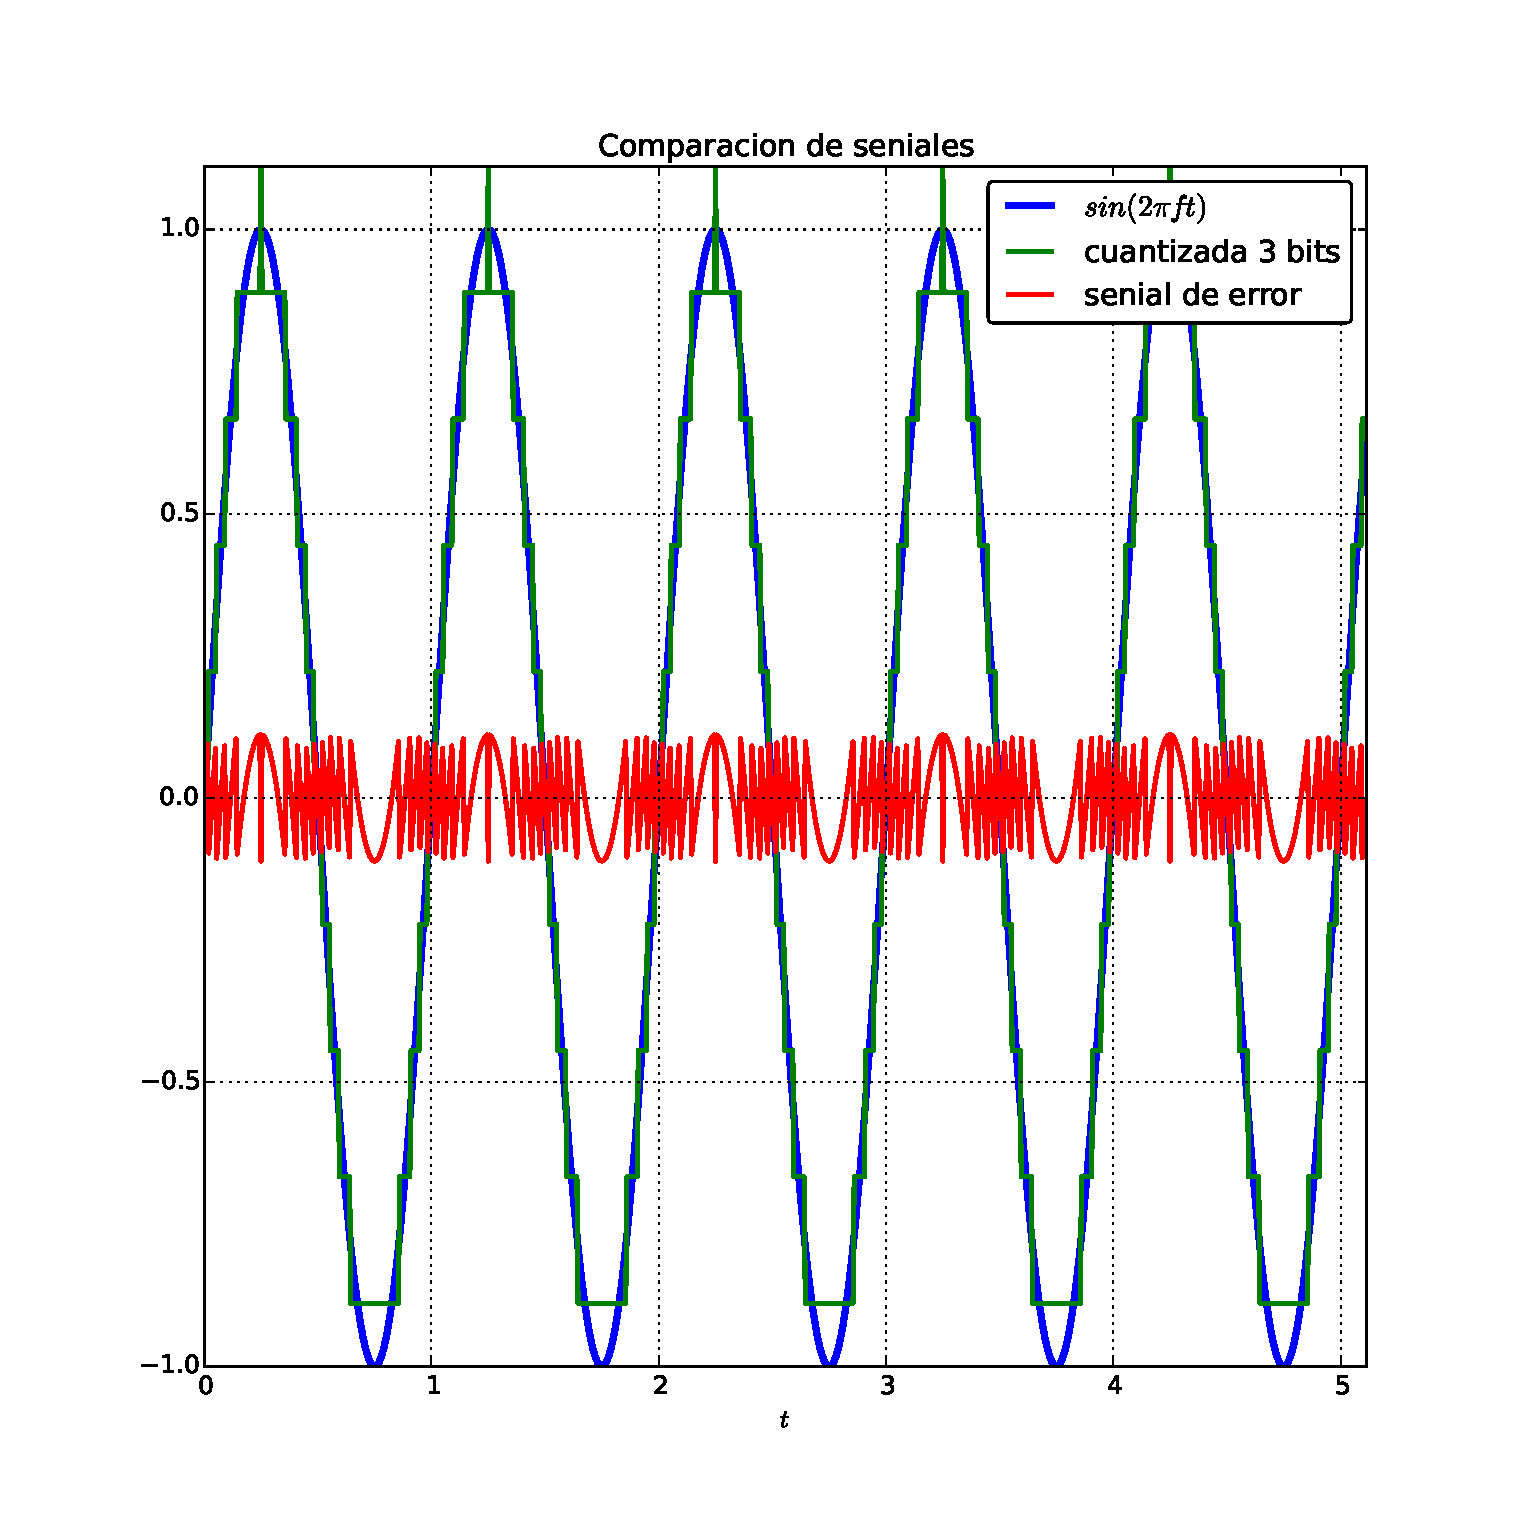
\includegraphics[width=0.78\textwidth]{./Images/seniales_3_bits.eps}
   \caption{Cuantización 3 bits}\label{fig:q:3}     
\end{figure}


\begin{figure}[H]
   \centering
   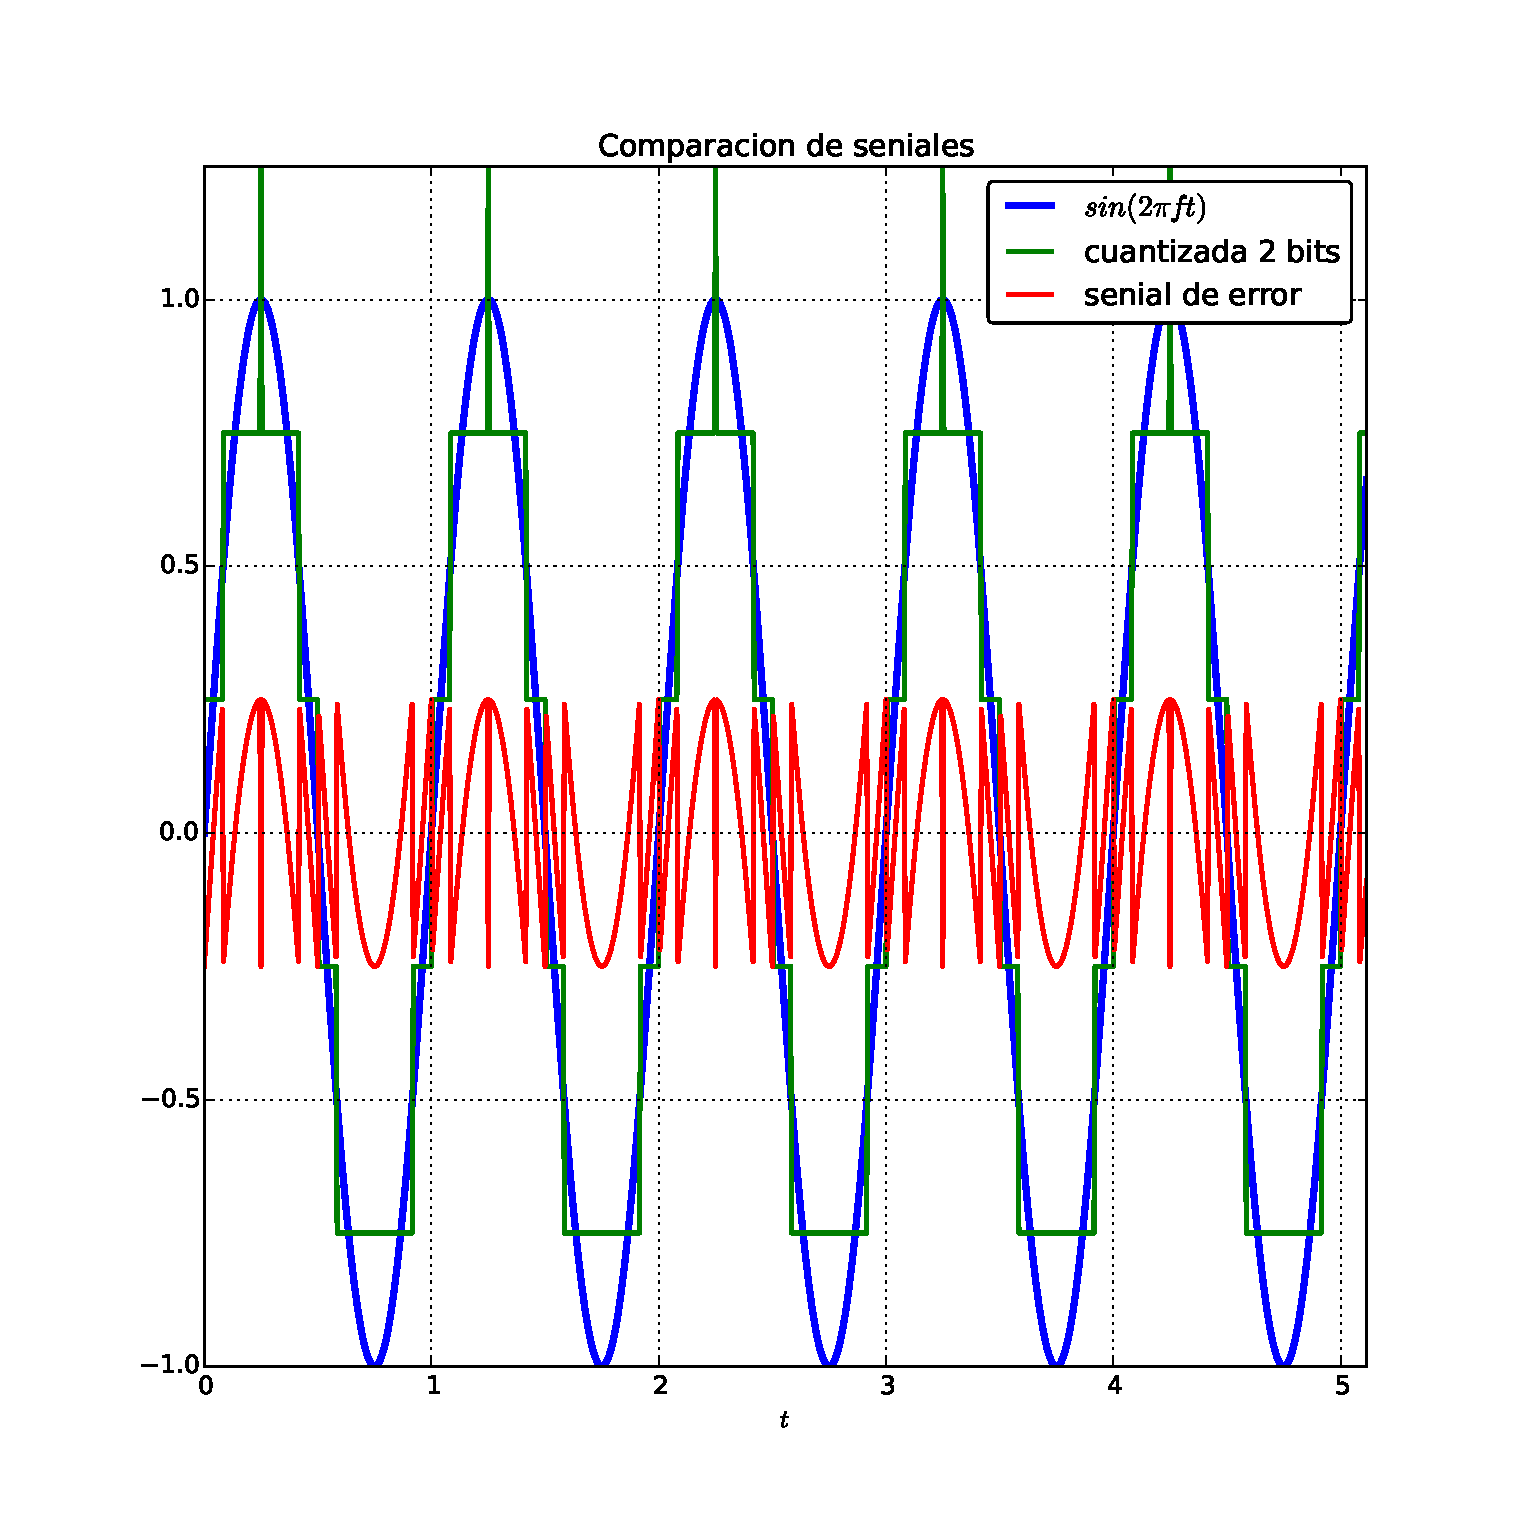
\includegraphics[width=0.78\textwidth]{./Images/seniales_2_bits.eps}
   \caption{Cuantización 2 bits}\label{fig:q:2}     
\end{figure}

Como se puede apreciar la señal de error $e(t)=x-x_{q_{i}}$ tiene amplitud más grande
al cuantizar a la señal original con menos niveles.

\section{Problema 5}
Se propone ahora simular los efectos de la cuantización uniforme sobre una señal
de voz (tomada de algún archivo de audio de pocos segundos de duración muestreada
con n bits de manera que su calidad sea media).
A partir de una señal de voz original se pide cuantizar la señal con menos bits que la
original

\begin{itemize}
    \item a- Medir la SNR para cada uno de los casos anteriores y reproducir la señal cuantizada en la tarjeta de audio. Comentar los resultados.
\end{itemize}

\subsection{resolución}
Nuevamente se realizó un script(\verb|problema5.jl|) que realiza la lectura-escritura de los archivos \verb|wav|
y además comparamos gráficamente todas las seniales. A continuación las salidas del mencionado script.


\begin{figure}[H]
   \centering
   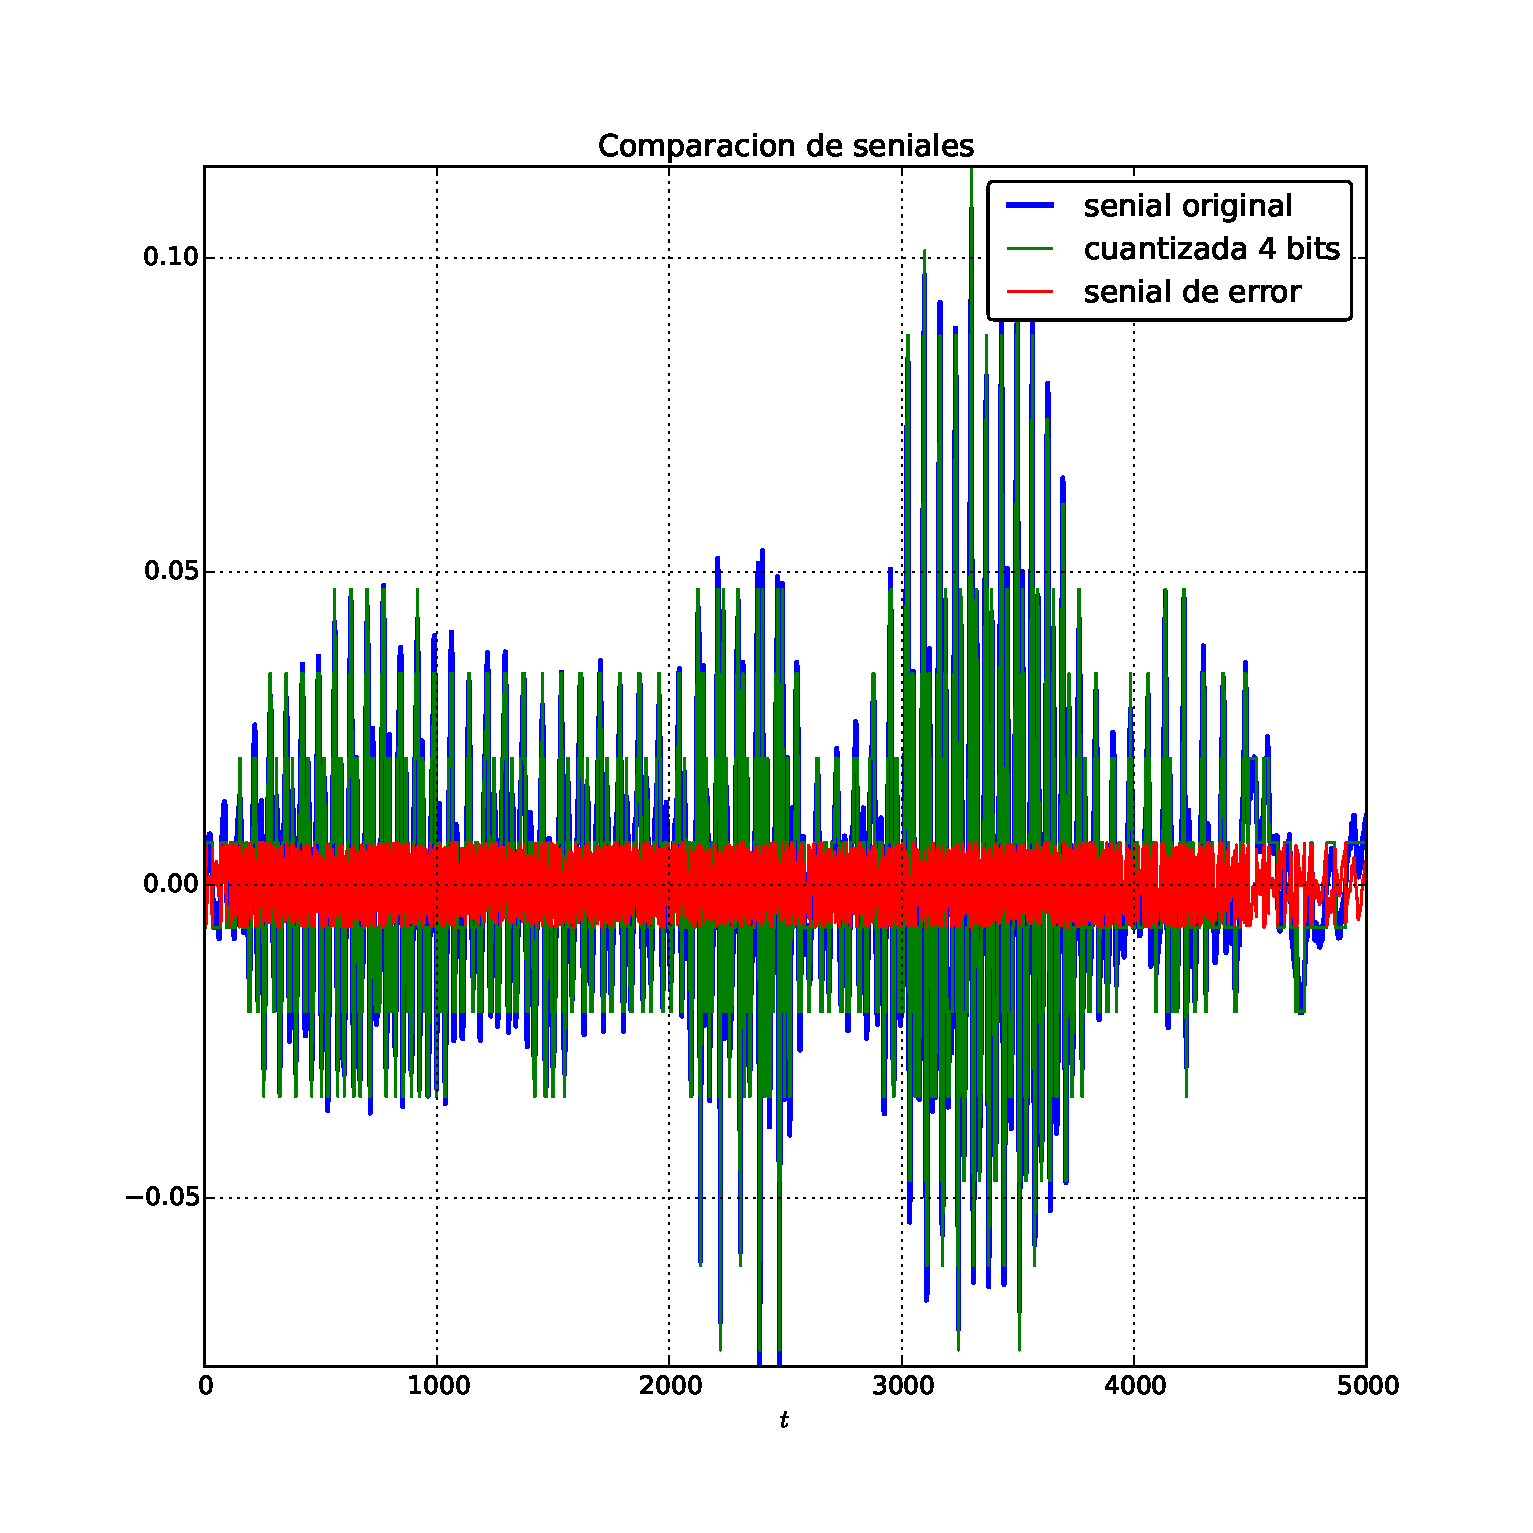
\includegraphics[width=0.78\textwidth]{./Images/senialesv_voz_4_bits.eps}
   \caption{Cuantización 4 bits}\label{fig:qv:4}     
\end{figure}


\begin{figure}[H]
   \centering
   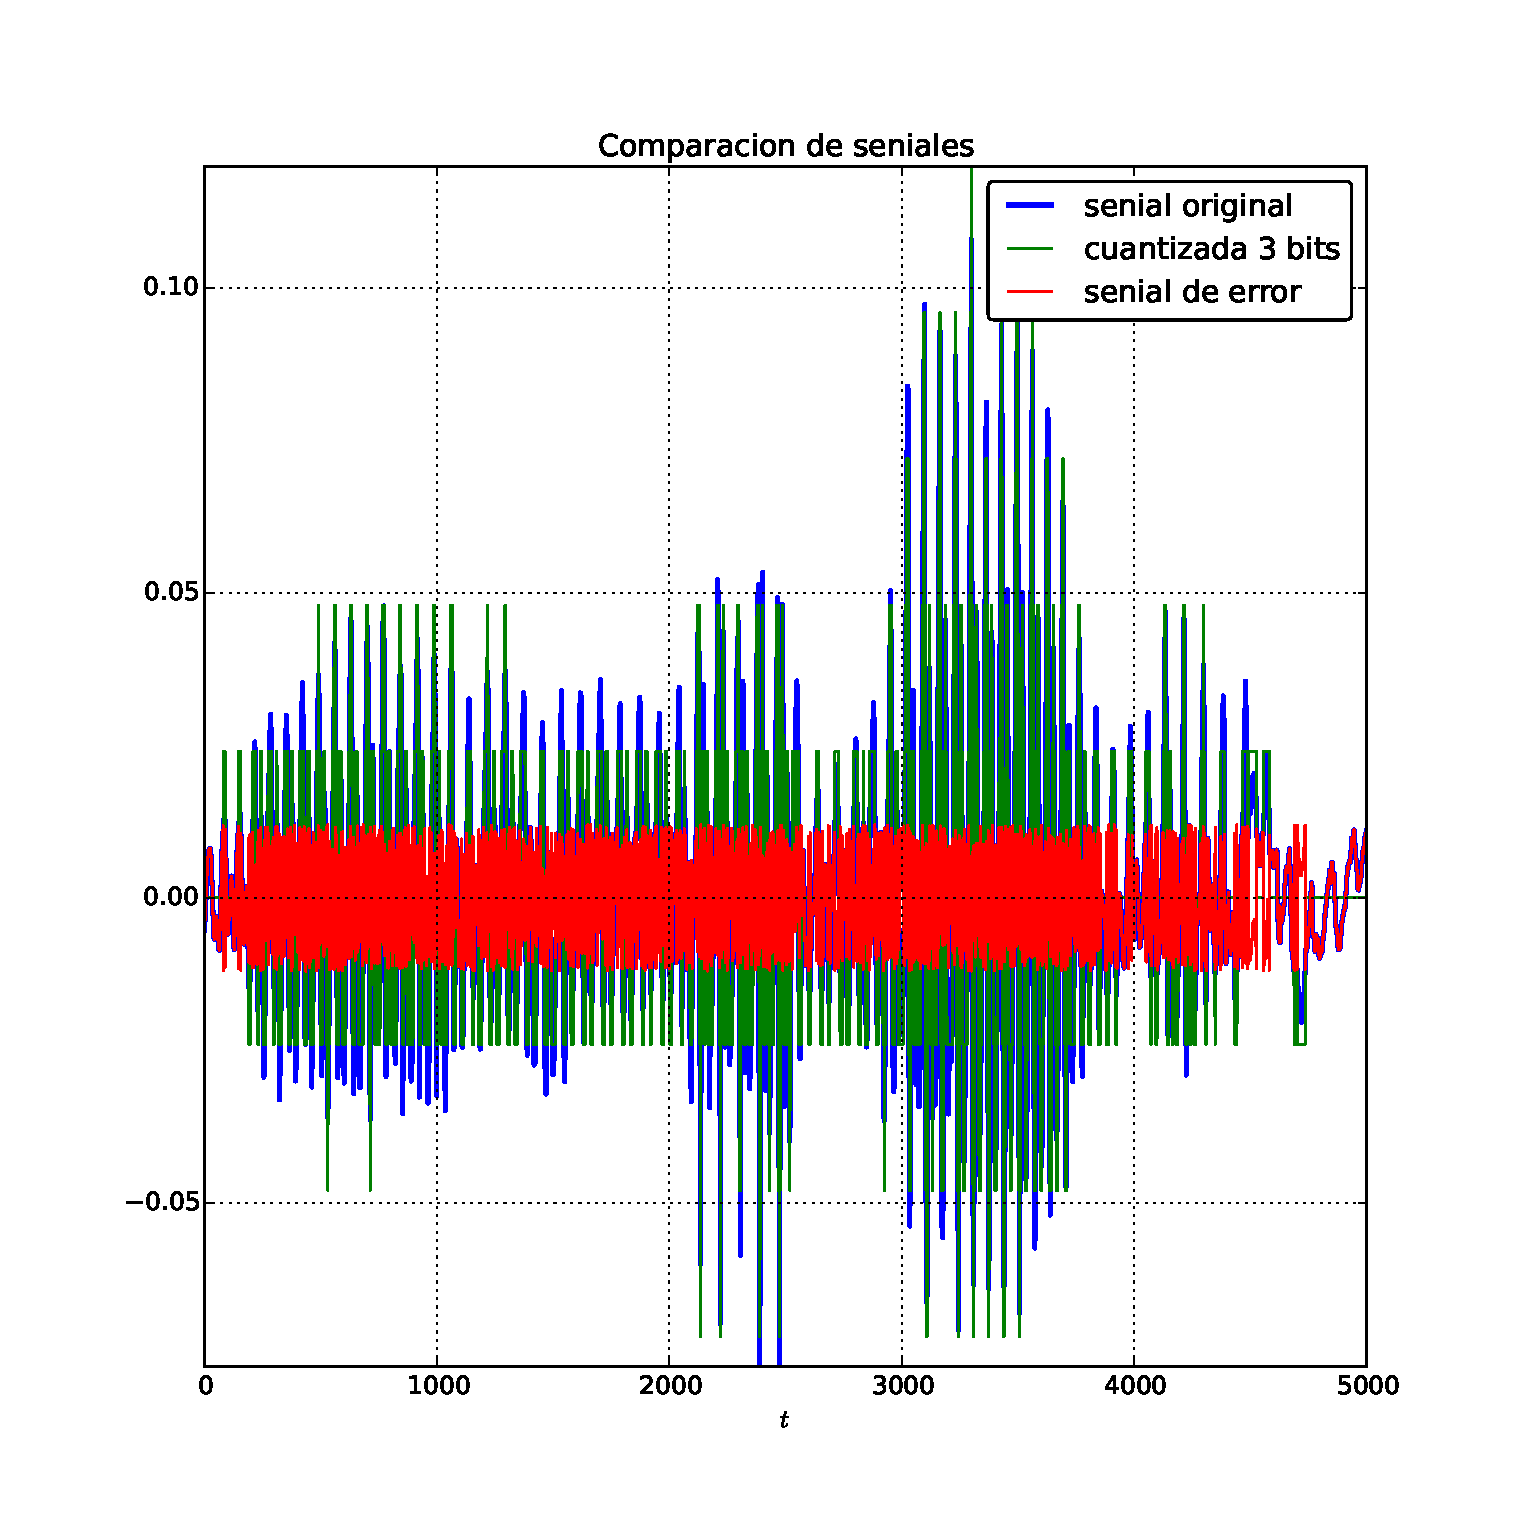
\includegraphics[width=0.78\textwidth]{./Images/senialesv_voz_3_bits.eps}
   \caption{Cuantización 3 bits}\label{fig:qv:3}     
\end{figure}


\begin{figure}[H]
   \centering
   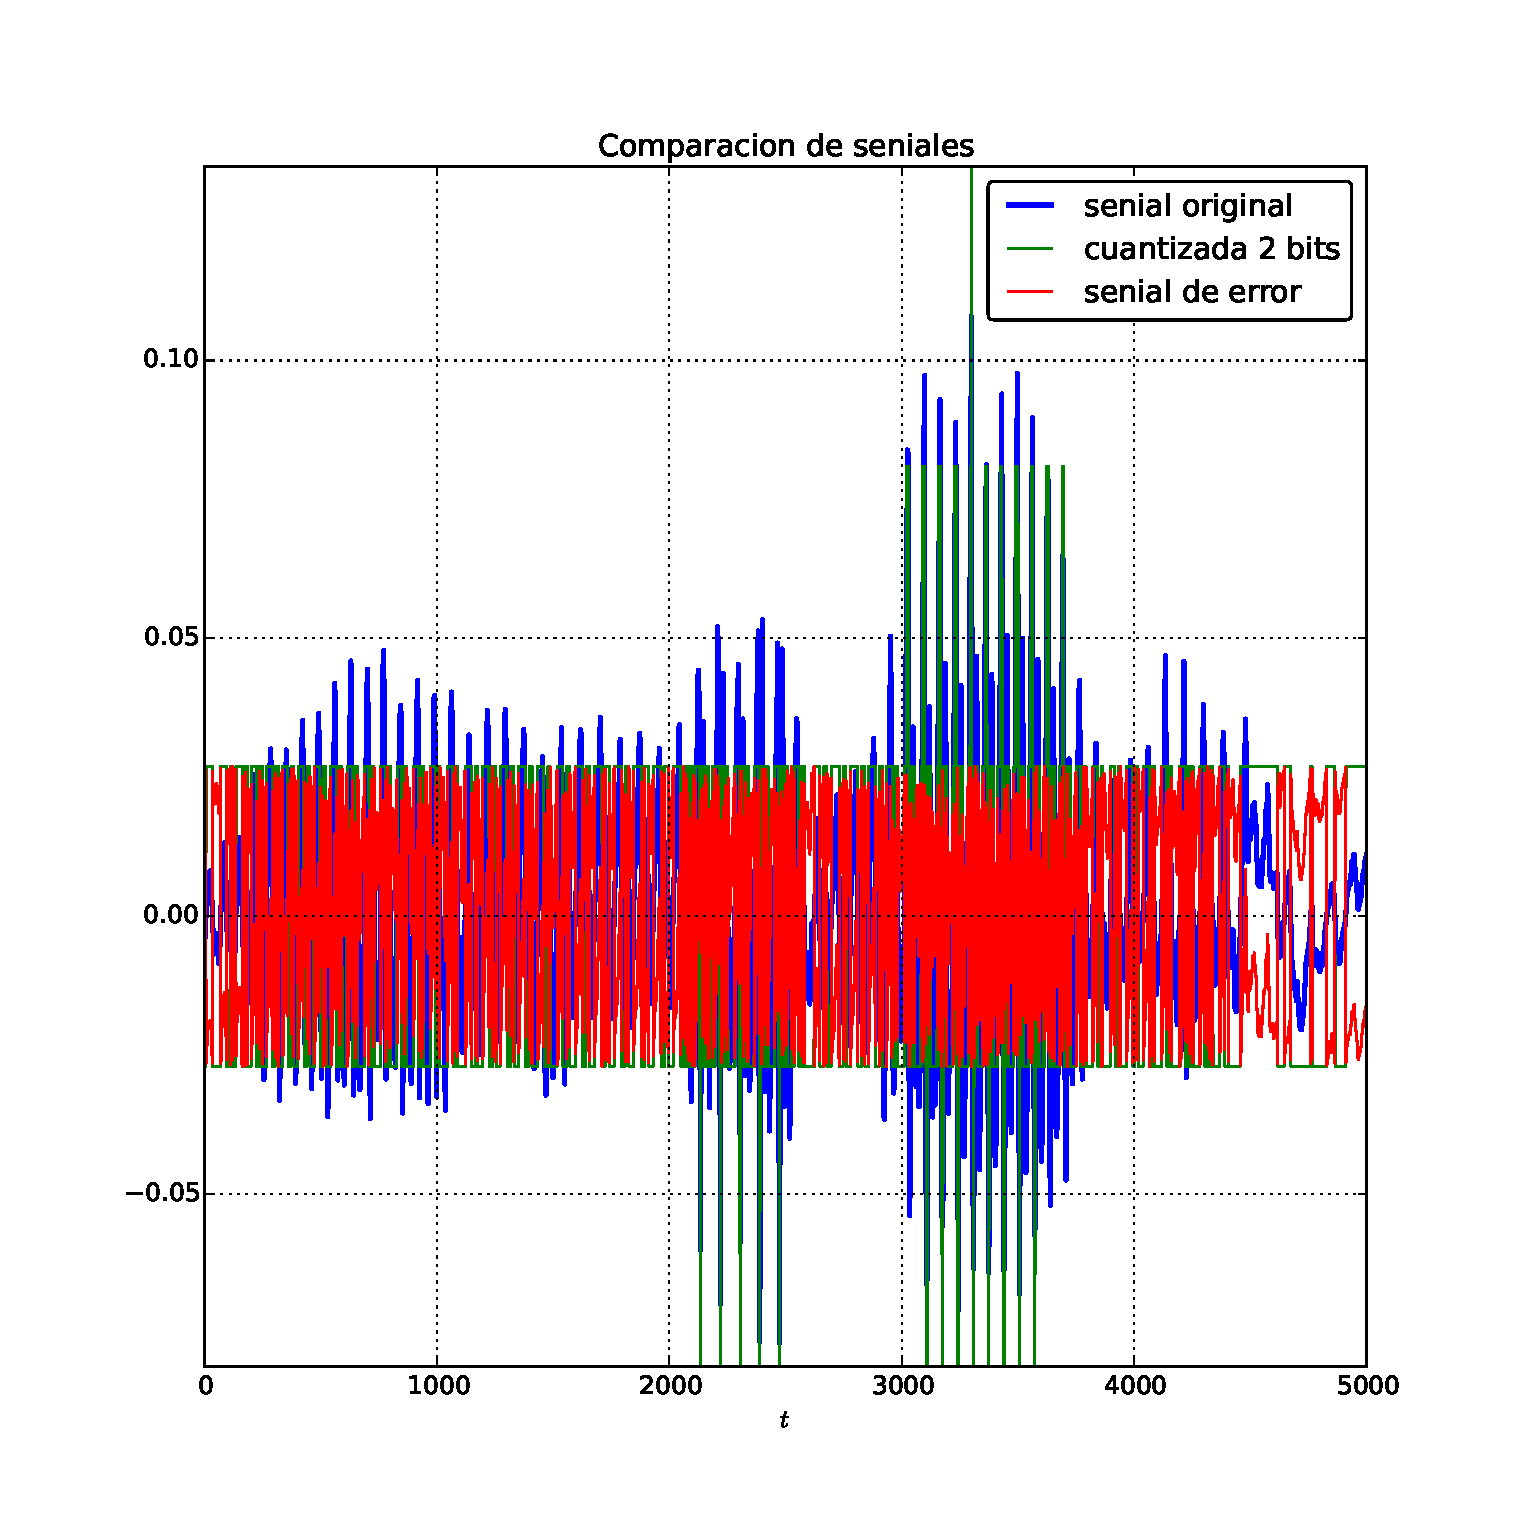
\includegraphics[width=0.78\textwidth]{./Images/senialesv_voz_2_bits.eps}
   \caption{Cuantización 2 bits}\label{fig:qv:2}     
\end{figure}
La relación senial-ruido para una senial cuantizada uniformemente se puede expresar:
\begin{equation}
\Bigg( \frac{S}{N} \Bigg)_{q} = \frac{L^{2}q^{2}/4}{q^{2}/12} = 3L^{2}
\end{equation}
Donde $L$ son los números de niveles de cuantización.

Por ello para 2 bits de resolución tenemos(en $[Db]$):

\verb|julia> 10*log10(12*1^2/2/(2/4)^2)|\\
\verb|13.80211241711606|\\
para 3 bits\\
\verb|julia>10*log10(12*1^2/2/(2/8)^2)|\\
\verb|19.822712330395685|\\
para 4 bits\\
\verb|julia>10*log10(12*1^2/2/(2/16)^2)|\\
\verb|25.84331224367531|\\

A la salida del script obtemos:
\begin{verbatim}
elsuizo@debian:~/Telecomunicaciones/Laboratorios/Lab1/Programas/Julia$ ~/julia/./julia problema5.jl 
INFO: Loading help data...
La relación senial-ruido para 2 bits es: 4.7383394267141[Db]
La relación senial-ruido para 3 bits es: 9.682605271481124[Db]
La relación senial-ruido para 4 bits es: 20.744776704544634[Db]
\end{verbatim}

Como sabemos las seniales de voz estadisticamente tienen amplitudes bajas, osea que
los niveles altos de voz son pocos probables, de alli que para esta senial de 
voz obtenemos resultados distintos de los teoricos que modelan a la probabilidad 
de $p(q)=1/q$ además si tomamos como indicador de como se
degrada la senial de acuerdo a la varianza del error producido por el redondeo, vimos que
la varianza $\sigma^{2}=\frac{q^{2}}{12}$ se corresponde con la potencia media de ruido 
a la cuantización. Por ello como podemos ver en la cuantización uniforme el ruido se mantiene constante
ya que $q$ es constante, pero como los niveles de amplitud no entonces la relación senial-ruido varía. 

\section{Problema 6}
Modificando el diagrama utilizado en la simulación de la cuantización uniforme para
señales de voz para implementar el cuantizador ley-$\mu$.
\begin{itemize}
\item a- Medir la SNR para cada uno de los casos (cuantización de 4, 3 y 2 bits) y
reproducir la señal cuantizada en la tarjeta de audio.
\item b- Modificar el esquema y adicionar dos “SCOPE”, uno antes de comprimir la
señal con un filtro con ley-$\mu$ y otro posterior al filtro con ley-$\mu$.
Sacar conclusiones en base a lo visualizado.
\item c- Comparar con los resultados del cuantizador uniforme y sacar
conclusiones.
\item d- Graficar la Densidad Espectral de la Señal (Utilizando Matlab) y Sacar
Conclusiones:
\begin{itemize}
\item A la entrada del Sistema.
\item A la salida del filtro ley-$\mu$.
\item A la salida del Sistema.
\end{itemize}
\end{itemize}
\subsection{resolución}

%-------------------------------------------------------------------------
% Bibliografia
%-------------------------------------------------------------------------

\begin{thebibliography}{6}
 \bibitem{Principal}{Digital communications, fundamentals and applications. Bernard Sklar}\\
 \bibitem{Principal2}{Julia: A fresh approach to numerical computing. Jeff Bezanson, Alan Edelman, Stefan Karpinski, Viral B. Shah(2014)}\url{http://arxiv.org/abs/1411.1607}
\end{thebibliography}

\end{document}
